\documentclass[12pt]{article}
\usepackage[margin=1in]{geometry}
\geometry{letterpaper}
\usepackage{amsmath}
\usepackage{amssymb}
\usepackage{graphicx}
\usepackage{amsfonts}
\usepackage{mathtools}
\usepackage{hyperref}
\usepackage[superscript]{cite}
% http://arxmliv.kwarc.info/package_usage.php

\begin{document}

\title{CS 51. Project Proposal.}
\date{Due April 10th, 2015.}
\author{Angela Fan, Andre Nguyen, Vincent Nguyen, George Zeng.}
\maketitle

\section{Basics}
We plan to work on a machine learning project with the ultimate goal of implementing a neural network by hand.

Our project members are:
\begin{itemize}
  \item Angela Fan \href{mailto:huihuifan@college.harvard.edu}
    {\nolinkurl{<huihuifan@college.harvard.edu>}}
  \item Andre Nguyen \href{mailto:andrenguyen@college.harvard.edu}
    {\nolinkurl{<andrenguyen@college.harvard.edu>}}
  \item Vincent Nguyen \href{mailto:vnguyen01@college.harvard.edu}
    {\nolinkurl{<vnguyen01@college.harvard.edu>}}
  \item George Zeng \href{mailto:gzeng@college.harvard.edu}
    {\nolinkurl{<gzeng@college.harvard.edu>}}
\end{itemize}

\section{Brief Overview}
As a group, we are very interested in learning more about machine learning methods. For this project, we would like to explore neural networks, as they have seen increasing use, particularly in deep learning.

We will implement a basic version of a Restricted Boltzmann Machine (RBM), a type of stochastic neural network that has been used in a variety of applications. Specifically, we are fascinated by the potential to apply neural networks to everyday pattern recognition in image recognition and classification. However, we will treat the goal of image recognition as an extension to our core project, a little something extra should we have time to explore it. 

Since implementing a successful RBM is a nontrivial task that cannot be modularized easily compared to other potential projects, our main goal for this final project is to successfully implement a working RBM. Doing so will entail many subtasks that are very interconnected in nature and hence our subgoals will be very abstract rather than concrete; in other words, we are not working towards specific checkpoints of completed subtasks. 

After successful implementation of our RBM by hand, we will have the opportunity to pursue further side-projects that are more ``extension''-oriented in the sense that each application and consequent tweaking of our RBM implementation will provide a very concrete representation. Moreover, if we can apply our RBM to image/pattern recognition project, we will have concrete visualizations and other physical demonstrations. 

We plan on implementing our project in Python because it is a very popular for machine learning. Python's high-level nature will allow us to focus on building abstractions rather than get distracted by low-level computational concerns. The version of Python we will be using will be Python 3 (not Python 2).

\section{Feature List}

We believe that implementing an RBM will be a decent amount of work. We will implement the RBM as well as a few functions to help assess its performance. We will train and test our RBM on a toy dataset of 10 users and the movies they like. 

We will explore the following extensions, time permitting:
\begin{enumerate}
  \item Persistent CD algorithm to approximate sampling from the energy function probability distribution, as an alternative to CD-k
  \item Train and test our RBM on more complicated datasets, such as MNIST handwriting image recognition and Faces in the Wild, a set of labeled images of faces
\end{enumerate}

\section{Technical Specification}

A restricted Boltzmann machine is a simplified version of a Boltzmann machine in which nodes at hidden layers are restricted to non-cyclical graphs. The RBM will tune the parameters of an energy-based probabilistic function (linear in its parameters) so that desirable states have lower energy configurations. The energy function will be defined as 
$$
E(v,h) = -b'v - c'h -h'Wv
$$ 
where $W$ represents the weights that connect the hidden and visible nodes, and $b$ and $c$ are offsets of the visible and hidden node layers.

We will then sample from the probability distribution generated by the energy function using a Gibbs Sampler. In order to speed up the sampling, we will use the Contrastive Divergence algorithm with $k=1$ (referred to as CD-$k$). The CD-$k$ algorithm speeds up the sampling because it does not wait for the markov chain to converge, and allows us to initialize the markov chain with a known training example, avoiding the potential burn-in time. $\diamond \diamond \diamond$

We will implement this project in an entirely object oriented fashion. We will be coding a class RBM that takes three parameters:
\begin{itemize}
  \item The number of hidden states
  \item The number of visible states
  \item A learning rate parameter
\end{itemize}

In the \texttt{init} function, the RBM will initialize a set of all weights that will be 0. Subsequently, we will use three methods:
\begin{itemize}
  \item The first method will just train the neural network, which will allow the network to traing weights
  \item The second method will take the trained RBM, run it on the visible units, and will yield a generated sample of hidden units
  \item The third method will be a hidden method--it will take a trained RBM, run it on the hidden units, and then generate the visible units
\end{itemize}

In the training phase, we will implement the CD-$k$ algorithm with $k = 1$ and update the bias layer of the network. 

From a slightly more modular/object-oriented point of view, our tasks consists of three components of the hierarchy:
\begin{itemize}
  \item At the bottom of the RBM we will have our individual units (``neurons'') which we can consider as the smallest building blocks of the RBM. The units will be either visible units or hidden units. Within each unit there will be some function which takes a vector as input and outputs binary values. In effect, we can think of the signature of a unit as containing at least a function and a value.
  \item Subsequently, we will build connection objects between the neurons. In the signatures for the the connection objects we specify two values: the value of the input neuron and the value of the output neuron.
  \item Once we have both connections and neurons, we will construct the greater neural network by building \textit{layers} using our units and connecting them. In particular, we will have visible layers (created by visible units) and hidden layers (created by hidden units).
\end{itemize}

\subsection{Project Responsibilities}
Our project will naturally split into the following components; we note that not all of these tasks are equivalent in terms of time and effort so that ultimately we will divide the responsibilities into subtasks such that magnitudes of time and effort are distributed equally among the group members:
\begin{itemize}
  \item Energy function
  \item Gibbs sampler
  \item CD-$k$ algorithm
  \item Contrastive divergence
  \item Writing the method to train the neural network
  \item Specifications of hidden states
  \item Specifications of visible states
  \item Determining hyperparameters
\end{itemize}

In addition to these individual subtasks, we will also work collectively as a group to debug the finished program as well as integrate and synthesize the various different modules of the task.

\begin{figure}
  \centerline{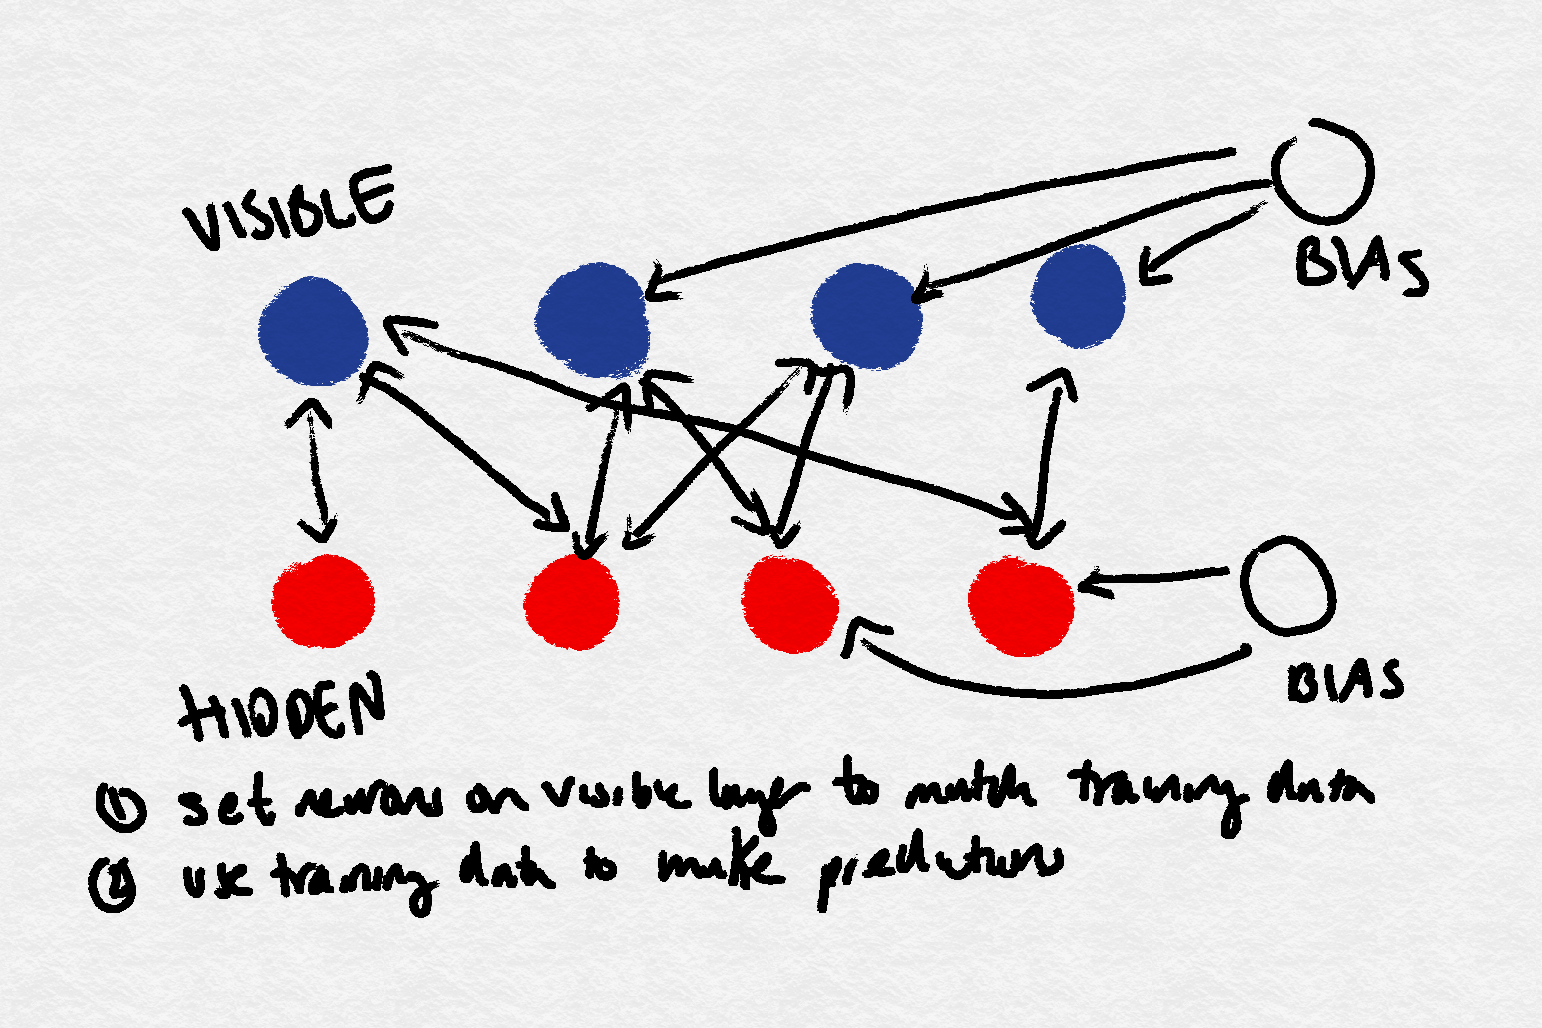
\includegraphics[scale=0.3]{layers_rbm.png}}
  \caption{Simple diagram of a neural network. To reiterate the hand-written captions above: we first intend to set the neurons on the visible layer to match training data, then we will use the training data to make predictions}
\end{figure}

\begin{figure}
  \centerline{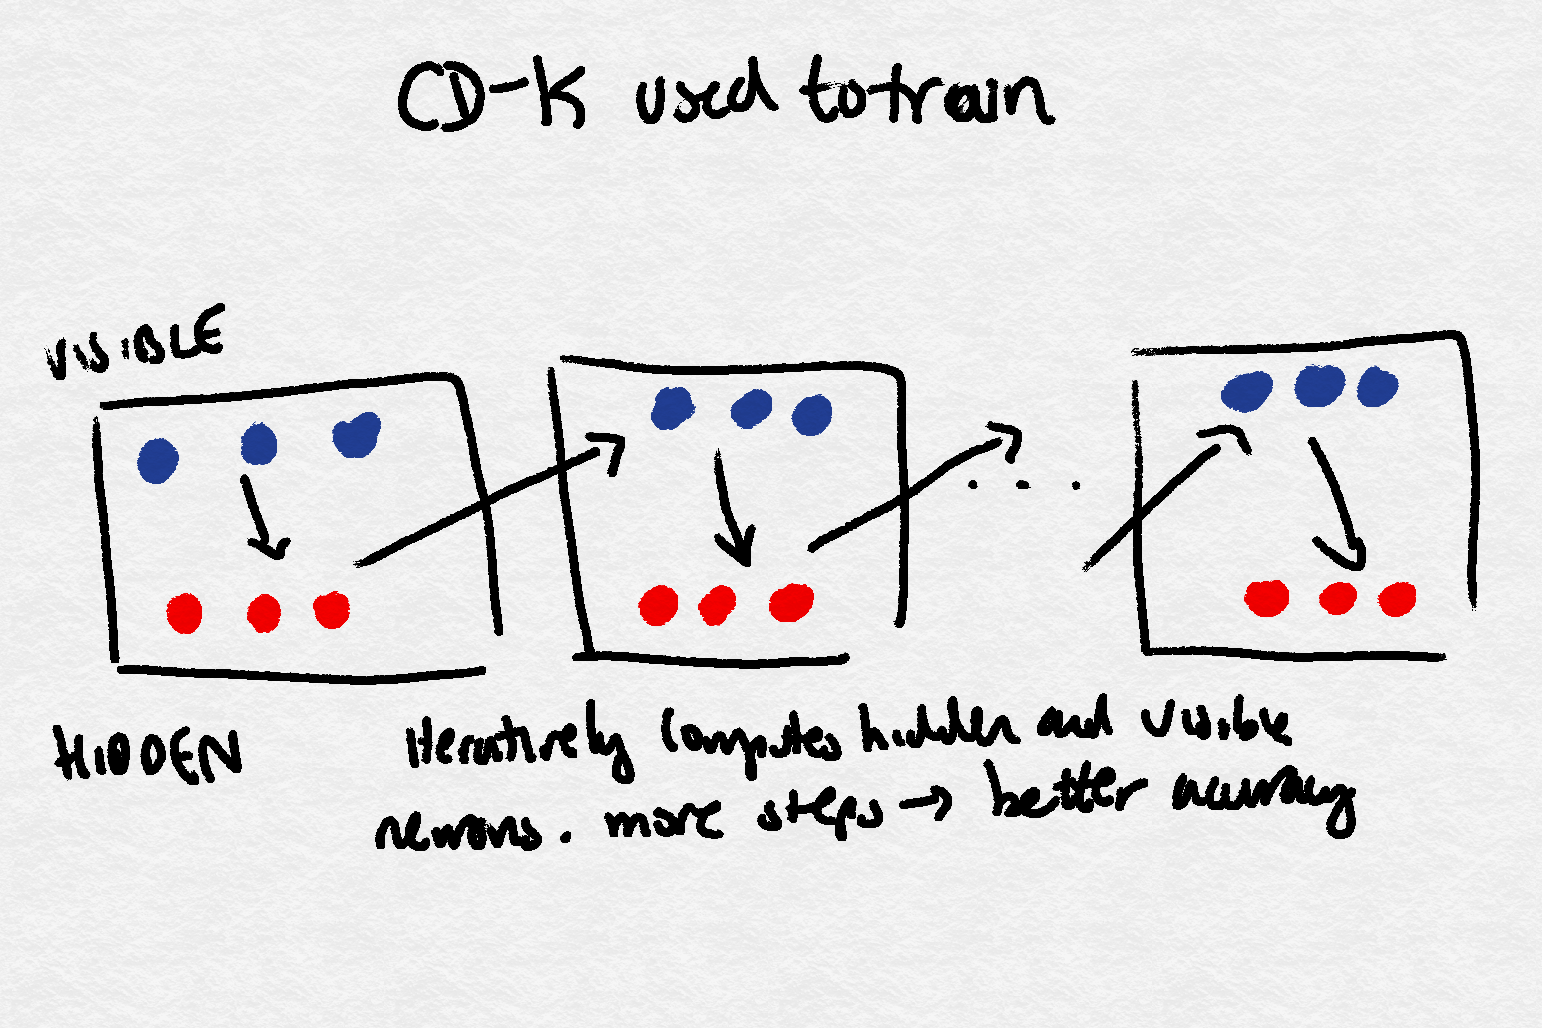
\includegraphics[scale=0.3]{cdk-1.png}}
  \caption{To reiterate the hand-written captions above: in using CD-$k$ to train, we iteratively computes hidden and visible neurons; a greater number of steps in the process will generally lead to greater accuracy in the final predictions. We can imaginge this process as each object's visible input is fed forward into the next object. }
\end{figure}

\section{Next Steps}

As an extension to our project, we intend to explore parameter optimization in the following ways:
\begin{itemize}
  \item Adjusting the learning rate parameter
  \item Adjusting the initial weights 
  \item Adjusting the initial biases
  \item Measuring and monitoring overfitting of the model
\end{itemize}

We will also explore the effects of using different types of units within the model. 

\end{document}
